\bluepage{Tessellation}

\begin{frame}[fragile]
\frametitle{OpenGL tessellation}
	\begin{itemize}
	\item Tessellation splits one primitive into more joint sub primitives.
	\item It can be used to refine details of a geometry.
	\item Tessellation is located between vertex shader and geometry shader.
	\item It is composed of three parts:
	\begin{itemize}
	\item Control Shader
	\item Primitive generation/tessellation
	\item Evaluation Shader
	\end{itemize}
	\item There is one new primitive type - \textcolor{red}{GL\_PATCHES}
	\end{itemize}
{\scriptsize
\begin{minted}[bgcolor=bg]{packages/c_cpp.py:CppLexer -x}
glPatchParameteri(GL_PATCH_VERTICES,10);//set number of vertices of patch to 10
glDrawArrays(GL_PATCHES,0,200);//draw 20 patches (each is composed of 10 vertices)
\end{minted}
}
	\begin{figure}[h]
	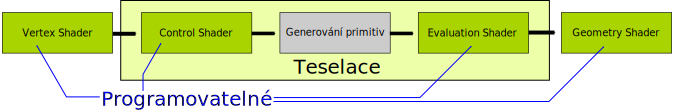
\includegraphics[width=10cm,keepaspectratio]{pics/tess_pipeline.pdf}
	\end{figure}
\end{frame}

\begin{frame}
\frametitle{Control Shader}
	\begin{itemize}
	\item CS controls level of tessellation.
	\item It computes control vertices.
	\item CS is invocated as many times as there is output vertices in output patch primitive.
	\item A invocation number is stored in built-in variable \textcolor{OliveGreen}{gl\_InvocationID}.
	\item We can synchronise threads in CS using \textcolor{OliveGreen}{barrier}().
	\end{itemize}
	\begin{figure}[h]
	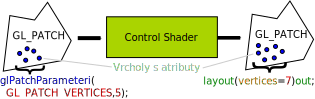
\includegraphics[width=10cm,keepaspectratio]{pics/tess_control.pdf}
	\end{figure}
\end{frame}

\begin{frame}
    \frametitle{Parameters}

    \includegraphics[width=\textwidth]{pics/tess.pdf}

    \begin{itemize}
				\item \textcolor{OliveGreen}{layout}
					(\{\textcolor{orange}{isolines},\textcolor{orange}{triangles},\textcolor{orange}{quads}\})
					\textcolor{OliveGreen}{in};
				\item \textcolor{OliveGreen}{gl\_TessLevelOuter}[4],\textcolor{OliveGreen}{gl\_TessLevelInner}[2]
    \end{itemize}
\end{frame}

\begin{frame}[fragile]
\frametitle{Control Shader - example}
{\scriptsize
\begin{minted}[bgcolor=bg]{packages/graphics.py:GLShaderLexer -x}
#version 430

// number of output vertices in output patch primitive ==
// number of threads per patch primitive
layout(vertices=3)out;

uniform vec2 TessLevelInner;//there are two inner and
uniform vec4 TessLevelOuter;//four outer levels of tessellation

void main(){
  //number of elements in gl_in depends on GL_PATCH_VERTICES
  //number of elements in gl_out delends on layout(vertices=n)out;
  //In this case, number of elements in gl_in and gl_out is the same.
  gl_out[gl_InvocationID].gl_Position=gl_in[gl_InvocationID].gl_Position;//copy
  if(gl_InvocationID==0){//the first thread sets tessellation levels
    gl_TessLevelOuter[0]=TessLevelOuter[0];
    gl_TessLevelOuter[1]=TessLevelOuter[1];
    gl_TessLevelOuter[2]=TessLevelOuter[2];
    gl_TessLevelOuter[3]=TessLevelOuter[3];
    gl_TessLevelInner[0]=TessLevelInner[0];
    gl_TessLevelInner[1]=TessLevelInner[1];
  }
}
\end{minted}
}
\end{frame}

\begin{frame}
\frametitle{Evaluation Shader}
	\begin{itemize}
		\item It sets type of tessellated primitive: \textcolor{Orange}{isolines},\textcolor{orange}{triangles},\textcolor{orange}{quads}
		\item It computes coordinates of tessellated vertices.
		\item \textcolor{OliveGreen}{gl\_TessCoord} variable holds barycentric, uv, or normalized coords of tessellated vertices inside of primitive.
		\item Evaluation shader is executed for every tessellated vertex.
		\item Tessellated primiteves continue their path to geometry shader.
	\end{itemize}
	\begin{figure}[h]
	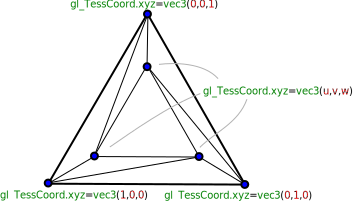
\includegraphics[width=7cm,keepaspectratio]{pics/tess_coord.pdf}
	\end{figure}
\end{frame}


\begin{frame}[fragile]
\frametitle{Evaluation Shader - example}
	\begin{itemize}
		\item Tessellated quad
		\item Computation of coordinates of tessellated vertices
	\end{itemize}
	{\scriptsize
\begin{minted}[bgcolor=bg]{packages/graphics.py:GLShaderLexer -x}
#version 430

layout(quads)in;

void main(){
  vec4 A=mix(gl_in[0].gl_Position,gl_in[1].gl_Position,gl_TessCoord.x);
  vec4 B=mix(gl_in[3].gl_Position,gl_in[2].gl_Position,gl_TessCoord.x);
  gl_Position=mix(A,B,gl_TessCoord.y);
}
	\end{minted}
	}
\end{frame}


\begin{frame}[fragile]
\frametitle{Béziér surface - example}
{\scriptsize
\begin{minted}[bgcolor=bg]{packages/graphics.py:GLShaderLexer -x}
// Vertex shader	
#version 430
void main() {
  gl_Position = mvp*position;
}

// Control shader
#version 430
layout(vertices=16) out;

void main() {
  gl_out[gl_InvocationID].gl_Position =
  gl_in[gl_InvocationID].gl_Position;
  if(gl_InvocationID == 0) {
    gl_TessLevelInner[0] = gl_TessLevelInner[1] = 
    gl_TessLevelOuter[0] = gl_TessLevelOuter[1] =
    gl_TessLevelOuter[2] = gl_TessLevelOuter[3] = 64;
  }
}
\end{minted}
}
\end{frame}

\begin{frame}[fragile]
  \frametitle{Béziér surface - example}
{\scriptsize
\begin{minted}[bgcolor=bg]{packages/graphics.py:GLShaderLexer -x}
// Evaluation shader
#version 430
layout(quads, ccw) in;

vec4 bernstein(float t) {
  return vec4((1-t)*(1-t)*(1-t), 3*t*(1-t)*(1-t), 3*t*t*(1-t), t*t*t);
}

void main() {
  vec4 bu = bernstein(gl_TessCoord.x);
  vec4 bv = bernstein(gl_TessCoord.y);
  vec4 position = vec4(0, 0, 0, 0);
  for(int y = 0; y < 4; ++y){
    for(int x = 0; x < 4; ++x){
      position += bu[x]*bv[y]*gl_in[4*y + x].gl_Position;
    }
  }
  gl_Position = position;
}
\end{minted}
}
\end{frame}

\begin{frame}[fragile]
\frametitle{Communication between shader stages}
{\tiny
\begin{minted}[bgcolor=bg]{packages/graphics.py:GLShaderLexer -x}
#version 430

//output vertex shader attributes
out vec4 vAttrib;
gl_Position

//intput control shader attributes
in  vec4 vAttrib[];//attribute from vertex shader, size == GL_PATCH_VERTICES
gl_in[].gl_Position;//a possition attribute from vertex shader

//output control shader attributes
out vec4 cAttrib[];//size == layout(vertices=size)out
patch out mat4 cM;//once per output patch primitive

//input evaluation shader attributes
in vec4 cAttrib[];//size == layout(vertices=size)out
patch in  mat4 cM;//once per input patch

//output evaluation shader attributes
out vec3 eNormal;

//input geometry shader attributes
in vec3 eNormal[];//size == 2 for line, size == 3 for triangle, ...
	\end{minted}
	}
\end{frame}

\begin{frame}[fragile]
    \frametitle{Example - replace triangles with circles}
  \begin{columns}[T]
    \begin{column}{.44\textwidth}
	    \begin{figure}[h]
    		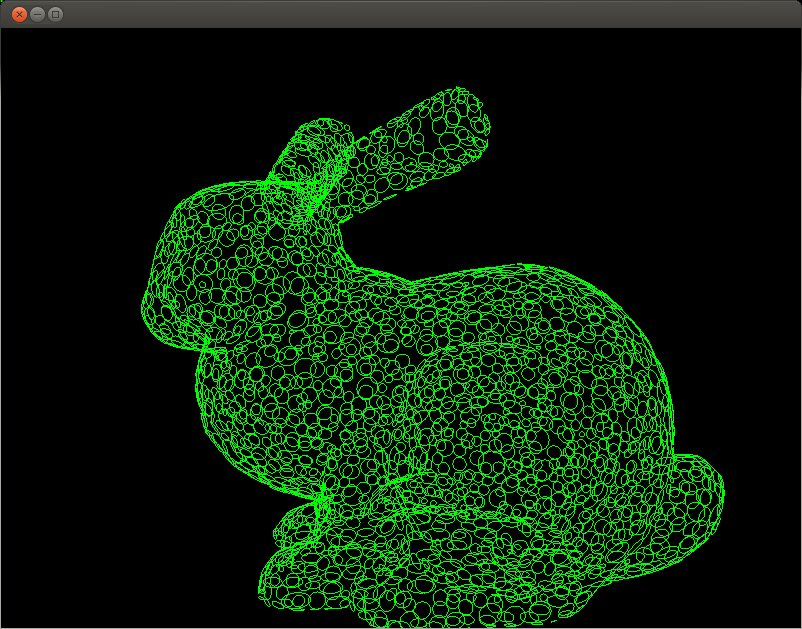
\includegraphics[width=5cm,keepaspectratio]{pics/ts_circle}
    	\end{figure}
    \end{column}
    \begin{column}{.48\textwidth}
 	    \begin{figure}[h]
    		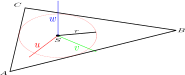
\includegraphics[width=5cm,keepaspectratio]{pics/circle.pdf}
    	\end{figure}
{\tiny
$$
K=
\left( 
\begin{array}{cccc} 
1 & 0 & 0 & S_x \\
0 & 1 & 0 & S_y \\
0 & 0 & 1 & S_z \\
0 & 0 & 0 & 1  \\
\end{array}
\right)
\cdot
\left( 
\begin{array}{cccc} 
r & 0 & 0 & 0 \\
0 & r & 0 & 0 \\
0 & 0 & r & 0 \\
0 & 0 & 0 & 1  \\
\end{array}
\right)
\cdot$$
$$
\left( 
\begin{array}{cccc} 
u_x & v_x & w_x & 0 \\
u_y & v_y & w_y & 0 \\
u_z & v_z & w_z & 0 \\
0 & 0 & 0 & 1  \\
\end{array}
\right)
$$
}
    \end{column}
  \end{columns}
\end{frame}

\begin{frame}[fragile]
    \frametitle{Example - replace triangles with circles}
  \begin{columns}[T]
    \begin{column}{.44\textwidth}
      Control Shader
{\tiny
\begin{minted}[bgcolor=bg]{packages/graphics.py:GLShaderLexer -x}
#version 400
layout(vertices=1)out;
patch out mat4 K;
void main(){
  gl_TessLevelOuter[0]=1;
  gl_TessLevelOuter[1]=64;
  gl_TessLevelOuter[2]=1;
  gl_TessLevelOuter[3]=1;
  gl_TessLevelInner[0]=1;
  gl_TessLevelInner[1]=1;
  vec4 TT[3];
  TT[0]=gl_in[0].gl_Position;
  TT[1]=gl_in[1].gl_Position;
  TT[2]=gl_in[2].gl_Position;
  float t01=length((TT[0]-TT[1]).xyz);
  float t02=length((TT[0]-TT[2]).xyz);
  float t12=length((TT[1]-TT[2]).xyz);
  float s=t01+t02+t12;
  float r=sqrt((s/2-t01)*(s/2-t02)*(s/2-t12)*s/2)*2/s;
  t01/=s;
  t02/=s;
  t12/=s;
  vec3 C=TT[0].xyz*t12+TT[1].xyz*t02+TT[2].xyz*t01;
  vec3 x=normalize(TT[0].xyz-C);
  vec3 y=normalize(TT[1].xyz-C);
  vec3 z=normalize(cross(x,y));
  y=normalize(cross(z,x));
  K=mat4(vec4(x,0)*r,vec4(y,0)*r,vec4(z,0)*r,vec4(C,1));
}
\end{minted}
}
    \end{column}
    \begin{column}{.48\textwidth}
      Evaluation Shader
{\tiny
\begin{minted}[bgcolor=bg]{packages/graphics.py:GLShaderLexer -x}
#version 400

#define MY_PI 3.14159265359

layout(isolines)in;

uniform mat4 V;
uniform mat4 P;

patch in mat4 K;

void main(){
  float Angle=gl_TessCoord.x*MY_PI*2;
  vec4 PP=vec4(cos(Angle),sin(Angle),0,1);
  gl_Position=P*V*K*PP;
}
\end{minted}
}
    \end{column}
  \end{columns}

\end{frame}


\begin{frame}
\frametitle{How to choose tessellation levels?}
	Outer level:
	\begin{itemize}
	\item Outer levels of edges of neighbor faces should be the same to prevent T-joints.
  \item Transform control points to the screen (screen-space distances).
	\item Divide edge length by maximal edge length.
	\end{itemize}
	Inner level:
	\begin{itemize}
	\item Average/maximum of outer levels
  \item ...
	\end{itemize}
\end{frame}

